% Original source: Zhou, physical PDF pp. 115--119 (printed pp. 99--103).
% Figures: Figure 4.7 and the ant-collision sketch redrawn natively with TikZ.
% Uncertainty log: none.

% ZHOU-SOURCE-PAGE: 115 PRINTED: 99

\[
\begin{aligned}
P(A\text{ or }B\text{ defaults})&=\E[I_A]+\E[I_B]-\E[I_AI_B]\\
&=\E[I_A]+\E[I_B]-\bigl(\E[I_A]\E[I_B]-\operatorname{cov}(I_A,I_B)\bigr)\\
&=0.5+0.3-\bigl(0.5\cdot0.3-\rho_{AB}\sigma_A\sigma_B\bigr)\\
&=0.65-\frac{\sqrt{0.21}}{2}\rho_{AB}
\end{aligned}
\]

For the maximum probability, we have
$0.65-\dfrac{\sqrt{0.21}}{2}\rho_{AB}=0.8\Rightarrow\rho_{AB}=-\sqrt{3/7}$.

For the minimum probability, we have
$0.65-\dfrac{\sqrt{0.21}}{2}\rho_{AB}=0.5\Rightarrow\rho_{AB}=\sqrt{3/7}$.

In this problem, do not start with
$P(A\text{ or }B\text{ defaults})=0.65-\dfrac{\sqrt{0.21}}{2}\rho_{AB}$ and try to set
$\rho_{AB}=\pm1$ to calculate the maximum and minimum probability since the correlation
cannot be $\pm1$. The range of correlation is restricted to
$\left[-\sqrt{3/7},\sqrt{3/7}\right]$.
\end{solution}

\subsection{Order Statistics}

Let $X$ be a random variable with cumulative distribution function $F_X(x)$. We can
derive the distribution function for the minimum $Y_n=\min(X_1,X_2,\ldots,X_n)$ and for
the maximum $Z_n=\max(X_1,X_2,\ldots,X_n)$ of $n$ IID random variables with \(\CDF\) $F_X(x)$
as

\begin{align*}
P(Y_n\geq x)&=(P(X\geq x))^n\\
&\Rightarrow1-F_{Y_n}(x)=(1-F_X(x))^n\\
&\Rightarrow f_{Y_n}(x)=nf_X(x)(1-F_X(x))^{n-1},\\
P(Z_n\leq x)&=(P(X\leq x))^n\\
&\Rightarrow F_{Z_n}(x)=(F_X(x))^n\\
&\Rightarrow f_{Z_n}(x)=nf_X(x)(F_X(x))^{n-1}.
\end{align*}

\begin{problem}{Expected value of max and min}

Let $X_1,X_2,\ldots,X_n$ be IID random variables with uniform distribution between 0 and
1. What are the cumulative distribution function, the probability density function and
expected value of $Z_n=\max(X_1,X_2,\ldots,X_n)$? What are the cumulative distribution
function, the probability density function and expected value of
$Y_n=\min(X_1,X_2,\ldots,X_n)$?

\end{problem}
\begin{solution}
This is a direct test of textbook knowledge. For uniform distribution on $[0,1]$,
$F_X(x)=x$ and $f_X(x)=1$. Applying $F_X(x)$ and $f_X(x)$ to
$Z_n=\max(X_1,X_2,\ldots,X_n)$ we have

\[
P(Z_n\leq x)=(P(X\leq x))^n\Rightarrow F_{Z_n}(x)=(F_X(x))^n=x^n
\]
\[
\Rightarrow f_{Z_n}(x)=nf_X(x)(F_X(x))^{n-1}=nx^{n-1}.
\]

% ZHOU-SOURCE-PAGE: 116 PRINTED: 100

and

\[
\begin{aligned}
\E[Z_n]&=\int_0^1xf_{Z_n}(x)\,\dd x=\int_0^1nx^n\,\dd x\\
&=\frac{n}{n+1}\left[x^{n+1}\right]_0^1=\frac{n}{n+1}.
\end{aligned}
\]

Applying $F_X(x)$ and $f_X(x)$ to $Y_n=\min(X_1,X_2,\ldots,X_n)$ we have

\[
P(Y_n\geq x)=(P(X\geq x))^n\Rightarrow F_{Y_n}(x)=1-(1-F_X(x))^n=1-(1-x)^n
\]
\[
\Rightarrow f_{Y_n}(x)=nf_X(x)(1-F_X(x))^{n-1}=n(1-x)^{n-1}
\]

and

\[
\begin{aligned}
\E[Y_n]&=\int_0^1nx(1-x)^{n-1}\,\dd x\\
&=\int_0^1n(1-y)y^{n-1}\,\dd y\\
&=\left[y^n\right]_0^1-\frac{n}{n+1}\left[y^{n+1}\right]_0^1=\frac{1}{n+1}.
\end{aligned}
\]
\end{solution}

\begin{problem}{Correlation of max and min}

Let $X_1$ and $X_2$ be IID random variables with uniform distribution between 0 and 1,
$Y=\min(X_1,X_2)$ and $Z=\max(X_1,X_2)$. What is the probability of $Y\geq y$ given
that $Z\leq z$ for any $y,z\in[0,1]$? What is the correlation of $Y$ and $Z$?

\end{problem}
\begin{solution}
This problem is another demonstration that a figure is worth a thousand words. As
shown in Figure 4.7, the probability that $Z\leq z$ is simply the square with side length
$z$. So $P(Z\leq z)=z^2$. Since $Z=\max(X_1,X_2)$ and $Y=\min(X_1,X_2)$, we must
have $Y\leq Z$ for any pair of $X_1$ and $X_2$. So if $y>z$,
$P(Y\geq y\vert Z\leq z)=0$. For $y\leq z$, that $X_1$ and $X_2$ satisfies $Y\geq y$
and $Z\leq z$ is the square with vertices $(y,y),(z,y),(z,z)$, and $(y,z)$, which has
an area $(z-y)^2$. So $P(Y\geq y\cap Z\leq z)=(z-y)^2$. Hence

\[
P(Y\geq y\vert Z\leq z)=
\begin{cases}
\dfrac{(z-y)^2}{z^2}, & \text{if }0\leq z\leq1\text{ and }0\leq y\leq z,\\
0, & \text{otherwise}.
\end{cases}
\]

Now let's move on to calculate the correlation of $Y$ and $Z$.

\[
\begin{aligned}
\operatorname{corr}(Y,Z)&=\frac{\operatorname{cov}(Y,Z)}{\operatorname{std}(Y)\cdot\operatorname{std}(Z)}\\
&=\frac{\E[YZ]-\E[Y]\E[Z]}{\sqrt{\E[Y^2]-\E[Y]^2}\cdot\sqrt{\E[Z^2]-\E[Z]^2}}.
\end{aligned}
\]

% ZHOU-SOURCE-PAGE: 117 PRINTED: 101

\begin{figure}[ht]
\centering
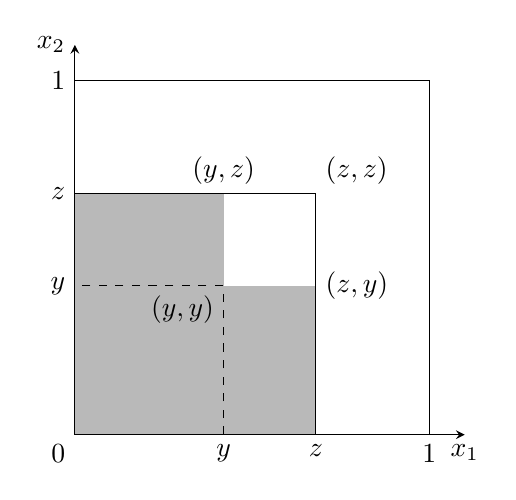
\begin{tikzpicture}[x=4.5cm,y=4.5cm,>=stealth]
  \coordinate (O) at (0,0);
  \coordinate (Y) at (0.42,0);
  \coordinate (Z) at (0.68,0);
  \coordinate (Ytop) at (0,0.42);
  \coordinate (Ztop) at (0,0.68);
  \fill[gray!55] (0,0) rectangle (0.68,0.68);
  \fill[white] (0.42,0.42) rectangle (0.68,0.68);
  \draw (0,0) rectangle (1,1);
  \draw (0,0.68) -- (0.68,0.68) -- (0.68,0);
  \draw[dashed] (0.42,0) -- (0.42,0.42) -- (0,0.42);
  \draw[->] (0,0) -- (1.1,0) node[below] {$x_1$};
  \draw[->] (0,0) -- (0,1.1) node[left] {$x_2$};
  \node[below left] at (O) {$0$};
  \node[below] at (Y) {$y$};
  \node[below] at (Z) {$z$};
  \node[left] at (Ytop) {$y$};
  \node[left] at (Ztop) {$z$};
  \node[left] at (0,1) {$1$};
  \node[below] at (1,0) {$1$};
  \node[above] at (0.42,0.68) {$(y,z)$};
  \node[above right] at (0.68,0.68) {$(z,z)$};
  \node[below left] at (0.42,0.42) {$(y,y)$};
  \node[right] at (0.68,0.42) {$(z,y)$};
\end{tikzpicture}
\caption{Distribution of $X_1$, $X_2$, their maximum and minimum.}
\label{fig:zhou-figure-4-7}
\end{figure}

Using previous problem's conclusions, we have $\E[Y]=\dfrac{1}{2+1}=\dfrac{1}{3}$,
$\E[Z]=\dfrac{2}{2+1}=\dfrac{2}{3}$. From the \(\PDF\)s of $Y$ and $Z$,
$f_Y(x)=n(1-x)^{n-1}=2(1-x)$ and $f_Z(z)=nz^{n-1}=2z$, we can also get
$\E[Y^2]=\int_0^1 2(1-y)y^2\,\dd y=\dfrac{2}{3}-\dfrac{2}{4}=\dfrac{1}{6}$ and
$\E[Z^2]=\int_0^1 2z^3\,\dd z=\dfrac{2}{4}$, which give us the variances:
$\operatorname{var}(Y)=\E[Y^2]-\E[Y]^2=\dfrac{1}{6}-\left(\dfrac{1}{3}\right)^2=\dfrac{1}{18}$
and $\operatorname{var}(Z)=\dfrac{2}{4}-\left(\dfrac{2}{3}\right)^2=\dfrac{1}{18}$.
\footnote[33]{You may have noticed that $\operatorname{var}(Y)=\operatorname{var}(Z)$ and wonder
whether it is a coincidence for $n=2$. It is actually true for all integer $n$. You may
want to think about why that is true without resorting to calculation. Hint:
$\operatorname{var}(x)=\operatorname{var}(1-x)$ for any random variable $x$.}

To calculate $\E[YZ]$, we can use
$\E[YZ]=\int_{\substack{0\le z\le1\\0\le y\le z}} yz f(y,z)\,\dd y\,\dd z$. To solve
this equation, we need $f(y,z)$. Let's again go back to Figure 4.7. From the figure we
can see that when $0\leq z\leq1$ and $0\leq y\leq z$, $F(y,z)$ is the shadowed area with
probability

\[
\begin{aligned}
F(y,z)&=P(Y\leq y\cap Z\leq z)=P(Z\leq z)-P(Y\geq y\cap Z\leq z)\\
&=z^2-(z-y)^2=2zy-y^2
\end{aligned}
\]
\[
\begin{aligned}
\therefore\quad f(y,z)&=\frac{\partial^2}{\partial y\,\partial z}F(y,z)=2
\\
\text{and}\quad \E[YZ]&=\int_{\substack{0\le z\le1\\0\le y\le z}}2yz\,\dd y\,\dd z\\
&=\int_0^1\left[zy^2\right]_0^z\,\dd z\\
&=\int_0^1z^3\,\dd z=\frac{1}{4}.
\end{aligned}
\]

% ZHOU-SOURCE-PAGE: 118 PRINTED: 102

An alternative and simpler approach to calculate $\E[YZ]$ is again to take advantage of
symmetry. Notice that no matter $x_1\leq x_2$ or $x_1>x_2$, we always have
$yz=x_1x_2$ ($z=\max(x_1,x_2)$ and $y=\min(x_1,x_2)$).

\[
\therefore\quad \E[YZ]=\int_{[0,1]^2}x_1x_2\,\dd x_1\,\dd x_2
=\E[X_1]\E[X_2]=\frac{1}{2}\cdot\frac{1}{2}=\frac{1}{4}.
\]

Hence $\operatorname{cov}(Y,Z)=\E[YZ]-\E[Y]\E[Z]=\dfrac{1}{36}$ and
$\operatorname{corr}(Y,Z)=\dfrac{\operatorname{cov}(Y,Z)}{\sqrt{\operatorname{var}(Y)}\cdot
\sqrt{\operatorname{var}(Z)}}=\dfrac{1}{2}$.

\emph{Sanity check:} That $Y$ and $Z$ have positive autocorrelation make sense since
when $Y$ becomes large, $Z$ tends to become large as well ($Z\geq Y$).
\end{solution}

\begin{problem}{Random ants}

500 ants are randomly put on a 1-foot string (independent uniform distribution for each
ant between 0 and 1). Each ant randomly moves toward one end of the string (equal
probability to the left or right) at constant speed of 1 foot/minute until it falls off at
one end of the string. Also assume that the size of the ant is infinitely small. When two
ants collide head-on, they both immediately change directions and keep on moving at 1
foot/min. What is the expected time for all ants to fall off the string?\footnote[34]{Hint: If we
switch the label of two ants that collide with each other, it's like that the collision never
happens.}

\end{problem}
\begin{solution}
This problem is often perceived to be a difficult one. The following components
contribute to the complexity of the problem: The ants are randomly located; each ant can
go either direction; an ant needs to change direction when it meets another ant. To solve
the problem, let's tackle these components.

\emph{When two ants collide head-on, both immediately change directions. What does it
mean?} The following diagram illustrates the key point:

\begin{center}
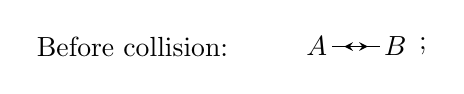
\begin{tikzpicture}[x=1cm,y=1cm,>=stealth,baseline=-0.5ex]
  \node[anchor=east] at (0,0) {Before collision:};
  \node at (1.00,0) {$A$};
  \node at (2.00,0) {$B$};
  \draw[->] (1.20,0) -- (1.65,0);
  \draw[<-] (1.35,0) -- (1.80,0);
  \node at (2.35,0) {;};
\end{tikzpicture}
\quad
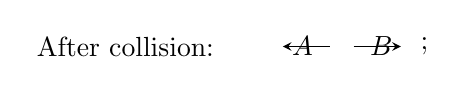
\begin{tikzpicture}[x=1cm,y=1cm,>=stealth,baseline=-0.5ex]
  \node[anchor=east] at (0,0) {After collision:};
  \node at (1.00,0) {$A$};
  \node at (2.00,0) {$B$};
  \draw[<-] (0.75,0) -- (1.35,0);
  \draw[->] (1.65,0) -- (2.25,0);
  \node at (2.55,0) {;};
\end{tikzpicture}
\quad
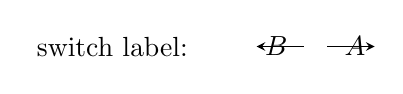
\begin{tikzpicture}[x=1cm,y=1cm,>=stealth,baseline=-0.5ex]
  \node[anchor=east] at (0,0) {switch label:};
  \node at (1.00,0) {$B$};
  \node at (2.00,0) {$A$};
  \draw[<-] (0.75,0) -- (1.35,0);
  \draw[->] (1.65,0) -- (2.25,0);
\end{tikzpicture}
\end{center}

When an ant $A$ collides with another ant $B$, both switch direction. But if we exchange
the ants' labels, it's like that the collision never happens. $A$ continues to move to the
right and $B$ moves to the left. Since the labels are randomly assigned anyway, collisions
make no difference to the result. So we can assume that when two ants meet, each just
keeps on going in its original direction. What about the random direction that each ant
chooses? Once the collision is removed, we can use symmetry to argue that it makes no
difference which direction that an ant goes either. That means if an ant is put at the
$x$-th foot, the

% ZHOU-SOURCE-PAGE: 119 PRINTED: 103

expected value for it to fall off is just $x$ min. If it goes in the other direction, simply set
$x$ to $1-x$. So the original problem is equivalent to the following:

What is the expected value of the maximum of 500 IID random variables with uniform
distribution between 0 and 1?

Clearly the answer is $\dfrac{499}{500}$ min, which is the expected time for all ants to fall
off the string.
\end{solution}
